%!TEX root = ../dokumentation.tex

\chapter{Grundlagen}
\section{Aussagenlogik}
Die klassische Aussagenlogik befasst sich mit Elementaraussagen (Atomen), denen ein Wahrheitswert zugeordnet wird. In der klassischen Aussagenlogik gibt es genau zwei Wahrheitswerte ``wahr'' und ``falsch''. Die Elementaraussagen können mittels Junktoren zu einer zusammengesetzten Aussage verknüpft werden. Eine solche zusammengesetzte Aussage hat ebenfalls einen Wahrheitswert, der sich über den Wahrheitswert der einzelnen Atome und die Junktoren berechnen lässt. Der Satz des ausgeschlossenen Dritten besagt, dass jedem Atom sowie jeder zusammengesetzte Aussage jeweils einer der zwei Wahrheitswerte zugeordnet werden muss. In der klassischen Logik gibt es also keine Unbestimmtheit über den Wahrheitswert einer Aussage. \cite{KB14}
\subsection{Induktive Formationsregeln}
Welche Aussagen in der klassischen Aussagenlogik formuliert werden können, wird über Formationsregeln induktiv definiert. Über die Menge der Atome $\psi$ lauten die Formationsregeln der Menge der Aussagen $\phi$ wie folgt \cite{SK18}:
\begin{itemize}
\item Alle atomaren Aussagen $\alpha\in\psi$ sind Aussagen in $\phi$.
\item \textbf{Negation}: Ist $\alpha$ eine Aussage von $\phi$, so auch $\neg\alpha$
\item \textbf{Konjunktion}: Sind $\alpha$ und $\beta$ Aussagen von $\phi$, so auch $\alpha\wedge\beta$
\item \textbf{Disjunktion}: Sind $\alpha$ und $\beta$ Aussagen von $\phi$, so auch $\alpha\vee\beta$
\item \textbf{Implikation}: Sind $\alpha$ und $\beta$ Aussagen von $\phi$, so auch $\alpha\rightarrow\beta$
\item \textbf{Äquivalenz}: Sind $\alpha$ und $\beta$ Aussagen von $\phi$, so auch $\alpha\leftrightarrow\beta$
\end{itemize}
Die Bedeutung der einzelnen Junktoren (Negation, Konjunktion, Disjunktion, Implikation, Äquivalenz) wird meist über sogenannte Wahrheitstabellen veranschaulicht \cite{KB14}.

\begin{table}
\begin{center}
\begin{tabular}{c|c}
$\alpha$ & $\neg\alpha$ \\
\hline
f & t \\
t & f
\end{tabular}
\end{center}
\caption{\label{tbl_neg}Wahrheitstabelle Negation}
\end{table}

Tabelle \ref{tbl_neg} zeigt die Wahrheitstabelle der Negation. In der linken Spalte werden die Wahrheitswerte der Aussage $\alpha$ dargestellt. Die rechte Spalte stellt entsprechend die Werte dar, nachdem $\alpha$ negiert, also der Junktor Negation angewandt wurde. Der einstellige Junktor ändert den Wahrheitswert der Aussage also immer in das ``Gegenteil'', wahr wird zu falsch und falsch zu wahr.

In der Tabelle \ref{tbl_prop_logic} ist die Wahrheitstabelle für die restlichen vorgestellten Junktoren dargestellt \cite{KB14}.
\begin{table}
\begin{center}
\begin{tabular}{c|c|c|c|c|c}
$\alpha$ & $\beta$ & $\alpha\wedge\beta$ & $\alpha\vee\beta$ & $\alpha\rightarrow\beta$ & $\alpha\leftrightarrow\beta$ \\
\hline
f & f & f & f & t & t \\
f & t & f & t & t & f \\
t & f & f & t & f & f\\
t & t & t & t & t & t\\
\end{tabular}
\end{center}
\caption{\label{tbl_prop_logic}Wahrheitstabelle Junktoren}
\end{table}

\subsection{\label{clamps_and_prio}Klammersetzung und Stelligkeit}
Ein wichtiger Aspekt der Aussagenlogik ist die Priorität der Junktoren. Ohne diese zu definieren würde es zu Ambiguitäten bei der Berechnung des Wahrheitswertes einer Aussage kommen. Ein Beispiel wäre die Aussage $\alpha\vee\beta\wedge\gamma$. Eine Möglichkeit diese Ambiguität zu verhindern, ist die Verwendung von Klammern. Der Wahrheitswert der Aussage, die innerhalb der Klammer steht, wird zuerst berechnet. Ohne Klammersetzung gäbe es für diese Aussage zwei unterschiedliche Möglichkeiten diese zu betrachten. Entweder als $(\alpha\vee\beta)\wedge\gamma$ oder als $\alpha\vee(\beta\wedge\gamma)$.

\begin{table}
\begin{center}
\begin{tabular}{c|c|c|c|c}
$\alpha$ & $\beta$ & $\gamma$ & $(\alpha\vee\beta)\wedge\gamma$ & $\alpha\vee(\beta\wedge\gamma)$ \\
\hline
f & f & f & f & f \\
f & f & t & f & f \\
f & t & f & f & f \\
f & t & t & t & t \\
t & f & f & f & t \\
t & f & t & t & t \\
t & t & f & f & t \\
t & t & t & t & t \\
\end{tabular}
\end{center}
\caption{\label{tbl_prop_prio}Wahrheitstabelle Beispiel Priorisierung}
\end{table}

Die Tabelle \ref{tbl_prop_prio} veranschaulicht den Unterschied in der Wahrheitswertezuweisung der beiden Interpretationen. Um diese Ambiguitäten bei der Kommunikation über Aussagen ohne Klammersetzung zu verhindern, wurden die Junktoren Priorisiert. Damit ist immer klar, welcher Junktor zuerst berechnet und damit was der Wahrheitswert einer Aussage ist. Die Prioritäten sind wie folgt definiert \cite{KB14}
\begin{enumerate}
\item Negation ($\neg$)
\item Konjunktion ($\wedge$)
\item Disjunktion ($\vee$)
\item Implikation ($\rightarrow$)
\item Äquivalenz ($\leftrightarrow$)
\end{enumerate}
Dieser Prioritätenfolge nach, wird obiges Beispiel also als $\alpha\vee(\beta\wedge\gamma)$ interpretiert.

\subsection{Tautologie und Kontradiktion}
Spezielle Aussageklassen sind Tautologien und Kontradiktionen. Diesen kann unabhängig der Wahrheitswerte der Atome, immer der Wahrheitswert wahr (Tautologie) oder falsch (Kontradiktion) zugewiesen werden. Das einfachste Beispiel für eine Tautologie wäre die Aussage $\alpha\vee\neg\alpha$. Für die Kontradiktion wäre das die Aussage $\alpha\wedge\neg\alpha$.

\section{Prädikatenlogik 1. Ordnung}
Eine Erweiterung der oben vorgestellten Aussagenlogik ist die Prädikatenlogik. Statt atomaren Aussagen, behandelt die Prädikatenlogik sogenannte Prädikate. Ein Prädikat stellt dabei eine Beziehung zu n Attributen dar, wobei n endlich und $n\in\N_{0}$. Der Satz ``Erna liebt Max'', stellt Beispielsweise das Prädikat ``liebt'' mit den Attributen Erna und Max dar. Die übliche Notation hierfür ist die Präfix, wodurch der Satz zu liebt(Erna, Max) wird \cite{KB14}.

\subsection{Quantoren}
Das Einführen von Attributen in die Prädikatenlogik ermöglicht es, Aussagen über eine Menge von Objekten zu machen. Z.B. $P(x_{0})\wedge$P$(x_{1})\wedge$...$\wedge$P$(x_{n})$. Mit den aktuellen Mitteln ist es allerdings nicht möglich eine solche Aussage für n=$\infty$ zu tätigen. Dafür werden in der Prädikatenlogik Quantoren eingeführt, mit denen Aussagen über alle möglichen Objekte getätigt werden können \cite{KB14}.
\begin{itemize}
\item
\textbf{Allquantor ($\forall$)} Eine Aussage mit einem Allquantor über die Variable x ist genau dann wahr, wenn x in der Aussage nach dem Allquantor durch jedes Objekt ersetzt werden kann und dann wahr ist.\\
Bsp.: $\forall$x P(x) $\leftrightarrow P(x_{0})\wedge$P$(x_{1})\wedge$...$\wedge$P$(x_{n})$ mit n=$\infty$.

\item
\textbf{Existenzquantor ($\exists$)} Eine Aussage mit einem Existenzquantor über die Variable x ist genau dann wahr, wenn x in der Aussage nach dem Existenzquantor durch mindestens ein Objekt ersetzt werden kann und dann wahr ist.\\
Bsp.: $\exists$x P(x) $\leftrightarrow P(x_{0})\vee$P$(x_{1})\vee$...$\vee$P$(x_{n})$ mit n=$\infty$.
\end{itemize}

\subsection{Induktive Formationsregeln}
Ähnlich der Aussagenlogik, sind korrekte prädikatenlogische Aussagen rekursiv definiert. Eine korrekte Aussage wird \ac{wff} genannt. Die Regeln lauten:
\begin{itemize}
\item
Prädikate mit der korrekten Anzahl Terme sind \ac{wff}. Z.B.: links(x), sieht(x,y), ...

\item
Ist $\alpha$ \ac{wff}, so ist auch $\neg\alpha$ \ac{wff}.

\item
Sind $\alpha$ und $\beta$ \ac{wff}, so sind auch $(\alpha\wedge\beta)$, $(\alpha\vee\beta)$, $(\alpha\rightarrow\beta)$ und $(\alpha\leftrightarrow\beta)$ alle \ac{wff}.

\item
Ist $\alpha$ \ac{wff}, so ist $\forall\nu\alpha$ und $\exists\nu\alpha$ auch \ac{wff} für jede Variable $\nu$.
\end{itemize}

Die in Abschnitt \ref{clamps_and_prio} definierten Prioritäten der Junktoren, trifft auch in der Prädikatenlogik zu. Für die Priorität der Quantoren gibt es leider keine feste Konvention, deshalb werden die Quantoren im Rahmen dieser Arbeit als am stärksten Bindend definiert. Dies führt zu folgender Prioritäten-folge:
\begin{enumerate}
\item Allquantor ($\forall$)
\item Existenzquantor ($\exists$)
\item Negation ($\neg$)
\item Konjunktion ($\wedge$)
\item Disjunktion ($\vee$)
\item Implikation ($\rightarrow$)
\item Äquivalenz ($\leftrightarrow$)
\end{enumerate}

\section{Intuitionistische Logik}
Die Intuitionistische oder auch nichtklassiche Logik ist ein anderes logisches Paradigma. Anstelle von wahren und falschen Aussagen und Atomen, behandelt die intuitionistische Logik beweisbare bzw. widerlegbare Aussagen und Atome. Beispielsweise wird die Aussage $\alpha\vee\neg\alpha$ in klassischer Logik als ``\textit{$\alpha$ trifft entweder zu, oder $\alpha$ trifft nicht zu}'' interpretiert. Die intuitionistische Interpretation lautet hingegen ``\textit{$\alpha$ ist beweisbar, oder $\alpha$ ist widerlegbar}''.

Dies klingt zuerst nach rein sprachlicher Formalität, hat aber einige Implikationen. Beispielsweise gilt der in klassischer Logik geltende Satz des ausgeschlossenen Dritten im Intuitionismus nicht. Der Satz des ausgeschlossenen Dritten besagt, dass jede Aussage entweder wahr oder falsch sein muss. Wie Gödel mit dem Gödelschen Unvollständigkeitssatz bewiesen hat, gibt es allerdings auch Aussagen die weder beweisbar noch widerlegbar sind \cite{B62}. 

Dies betrifft nicht nur Aussagen, die weder beweisbar noch nicht beweisbar sind sondern kann auch als ``Weder $\alpha$ noch $\neg\alpha$ konnten bis heute bewiesen werden'', interpretiert werden. Die Ungültigkeit des Satzes vom ausgeschlossenen Dritten hat einige Implikationen \cite{B62}
\begin{itemize}
\item Die Aussage $\alpha\vee\neg\alpha$, welche in klassischer Aussagenlogik eine Tautologie ist, ist im Intuitionismus keine.

\item Eine doppelte Negation ($\neg\neg\alpha$), ist nicht Äquivalent zur Aussage ohne Negation ($\alpha$). Die doppelte Negation von $\alpha$ im Intuitionismus bedeutet ``\textit{Es ist nicht beweisbar, dass $\alpha$ nicht beweisbar ist.}'' was nicht Äquivalent zu ``\textit{$\alpha$ ist beweisbar}'' ist.
\end{itemize}

Dieses logische Paradigma ist insbesondere zur mathematischen Schlussfolgerung, bei der aus bewiesenen Sätzen auf andere Sätze geschlossen, d.h. andere Sätze bewiesen werden sinnvoll. Dementsprechend ist die zugrundeliegende Denkweise bei der Implikation in der intuitionistischen Logik eine andere.

\subsection{\label{impl_in_intu}Implikation im Intuitionismus}
Eine Implikation $\alpha\rightarrow\beta$, kann im Intuitionismus als ``\textit{Wenn $\alpha$ beweisbar ist, kann daraus ein Beweis für $\beta$ abgeleitet werden.}'', betrachtet werden. Im Vergleich dazu, lautet die klassische Interpretation ``\textit{Wenn $\alpha$ zutrifft, dann trifft $\beta$ zu.}'' \cite{B62}.

Für die Tableau-Bildung hat dies eine ganz andere Betrachtungsweise zur Folge wie im Abschnitt \ref{tableaux_impl_descr} erarbeitet wird.

\subsection{\label{intu_non_proof_sentence}Nicht beweisbarer Satz $\perp$}
Die einzige Anpassung der Syntax, die von klassischer Aussagenlogik zur nichtklassischen Aussagenlogik bzw. von klassischer Prädikatenlogik zu nichtklassischer Prädikatenlogik vorgenommen werden muss, ist die Einführung eines nicht beweisbaren Satzes $\perp$. Dies ist für die Behandlung von Negationen in Tableaux notwendig. Der Satz $\neg\alpha$ ist Äquivalent zu $\alpha\rightarrow\perp$. Wenn ein Beweis für $\alpha$ gefunden werden kann, ist daraus auch ein Beweis für $\perp$ abgeleitet werden. Da es per Definition keinen Beweis für $\perp$ geben kann, ist dies Äquivalent zur Nichtbeweisbarkeit von $\alpha$ \cite{DGHP99}.

Zudem ist der Satz $\perp\rightarrow\alpha$ für jedes $\alpha$ immer beweisbar. Denn wenn ein Beweis für $\perp$ gefunden werden kann, kann daraus ein Beweis für jede andere Aussage abgeleitet werden \cite{DGHP99}.

\section{Tableaux}
Ein Tableau ist eine beweistheoretische Entscheidungsmethode, mit der in verschiedenen Logiken eine Aussage auf Gültigkeit, also auf Tautologie, mit berechenbaren Schritten geprüft werden kann \cite{DGHP99}. In den folgenden Abschnitten werden Tableaux für die oben vorgestellten Logiken vorgestellt.

Ein Tableau, in der in dieser Arbeit verwendeten Variante nach \cite{BK82}, besteht aus zwei Seiten. In klassischer Logik sind diese die Wahr- und die Falsch-Seite. In nichtklassischer wären diese Annahmen und Folgerungen. Auf den beiden Seiten befinden sich jeweils Aussagen, aus denen mit definierten Regeln weitere Aussagen auf den beiden Seiten erzeugt werden. Wurden die Regeln auf eine Aussage angewandt, ist diese abgearbeitet und wird im weiteren Verlauf der Abarbeitung nicht mehr betrachtet (Nicht immer siehe z.B. \ref{tableaux_classic_pred}).

Allgemein wird ein Tableau immer durch induktive Anwendung von Ableitungsregeln gebildet. Die Regeln und zu betrachtende Nebenbedingungen unterscheiden sich dabei allerdings in den einzelnen Logiken.

\subsection{Klassische Aussagenlogik}
Die Regeln, nach denen ein Tableau in klassischer Aussagenlogik gebildet wird, können wie folgt hergeleitet werden. Wird eine Aussage $\gamma$ betrachtet, wird der Junktor, sowie die Aussage(n) aus denen sich $\gamma$ zusammensetzt angeschaut. Je nach Seite (wahr/falsch) wird nun betrachtet, welche Werte die einzelnen Aussagen annehmen müssen, um den Wert der Seite (wahr/falsch) zu erzeugen. Die Regeln leiten sich also direkt aus den Wahrheitstabellen (\ref{tbl_prop_logic}) ab.

Betrachten wir beispielsweise die Aussage $\alpha\wedge\beta$ auf der Wahr-Seite. Nach Wahrheitstabelle \ref{tbl_prop_logic}, muss sowohl $\alpha$ als auch $\beta$ den Wahrheitswert wahr annehmen, damit die Aussage wahr ist. Es wird also sowohl $\alpha$, als auch $\beta$ auf die Wahr-Seite geschrieben. Um die Abarbeitung der Aussage zu notieren, wird diese unterstrichen \cite{KB14}. Siehe Abbildung \ref{tableaux_prop_and}.

\begin{figure}
\begin{center}
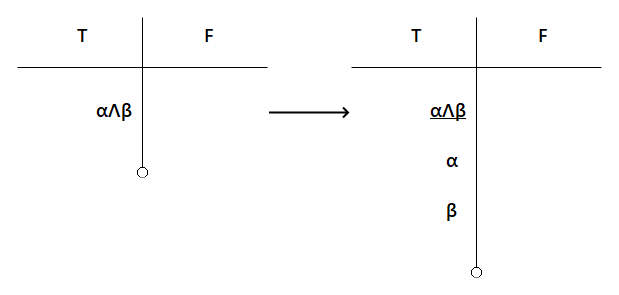
\includegraphics[scale=0.7]{images/Tableaux_And_Prop_Logic.png}
\caption{Tableaux der Aussage $\alpha\wedge\beta$ in klassischer Logik. Links: Tableau vor Anwendung der Ableitungsregel. Rechts: Tableau nach Anwendung der Ableitungsregel.}
\label{tableaux_prop_and}
\end{center}
\end{figure}

Damit kann schon der Großteil der Ableitungsregeln hergeleitet werden. Eine Ausnahme stellt die Situation dar, bei der beispielsweise $\alpha\vee\beta$ auf der Wahr-Seite steht. Es gibt mehrere Möglichkeiten mit denen diese Aussage wahr wird. Es kann entweder $\alpha$ oder $\beta$ wahr sein. In einer solchen Situation wird das Tableau in zwei voneinander unabhängige Pfade aufgeteilt. In beiden müssen alle noch nicht abgearbeiteten Aussagen unabhängig voneinander abgearbeitet werden. Siehe Abbildung \ref{tableaux_prop_or}. Die übrigen Ableitungsregeln sind in Abbildung \ref{tableaux_class_prop_all_rules} dargestellt.

\begin{figure}
\begin{center}
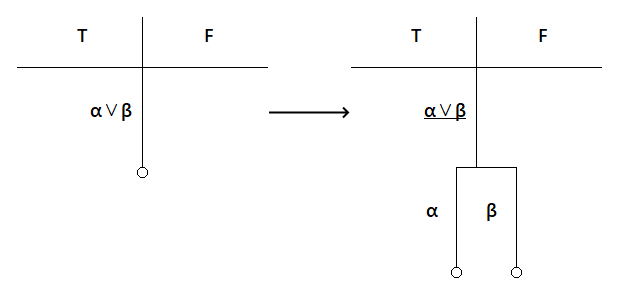
\includegraphics[scale=0.7]{images/Tableaux_Or_Prop_Logic.png}
\caption{Tableaux der Aussage $\alpha\vee\beta$ in klassischer Logik. Links: Tableau vor Anwendung der Ableitungsregel. Rechts: Tableau nach Anwendung der Ableitungsregel.}
\label{tableaux_prop_or}
\end{center}
\end{figure}

\begin{figure}
\begin{center}
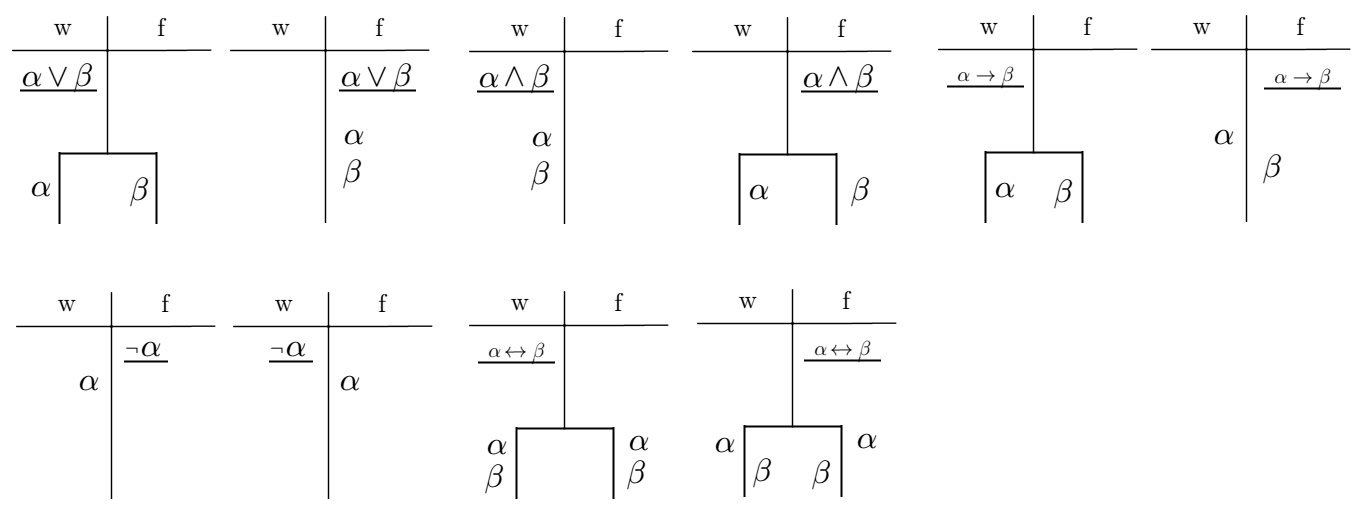
\includegraphics[scale=0.5]{images/Tableaux_Rules_Prop_Logic.png}
\caption{Tableaux Ableitungsregeln in klassischer Aussagenlogik}
\label{tableaux_class_prop_all_rules}
\end{center}
\end{figure}

Die Ableitungsregeln werden wiederholt, bis keine weiteren nicht abgearbeiteten Aussagen (nicht unterstrichen) übrig sind, oder eine Aussage sowohl auf der Wahr- als auch auf der Falsch-Seite steht. In einem solchen Fall, gilt der Pfad als geschlossen und wird mit einem doppelten Unterstrich unter der Trennlinie zwischen den beiden Seiten dargestellt. Sind alle Pfade eines Tableau geschlossen, wurde damit bewiesen, dass es keine Möglichkeit gibt, mit der die ursprüngliche Aussage den gegebenen Wahrheitswert annimmt. Will man also eine Aussage auf Tautologie untersuchen, beginnt man mit der Aussage auf der Falsch-Seite, schließt das Tableau wurde durch Kontradiktion bewiesen, dass die Aussage eine Tautologie ist. Bleibt ein Pfad offen, so wurde ein Gegenbeispiel durch die Atome auf der Wahr- und Falsch-Seite konstruiert \cite{KB14}.

\subsection{\label{tableaux_classic_pred}Klassische Prädikatenlogik 1. Ordnung}
Da die klassische Prädikatenlogik 1. Ordnung eine Erweiterung der Aussagenlogik ist, können die in Abbildung \ref{tableaux_classic_pred} vorgestellten Regeln dafür ebenfalls angewandt werden. Die Quantoren benötigen allerdings eine gesonderte Betrachtung. Zur einfacheren Behandlung dieser Regeln führen wir folgende Notation ein ``$\alpha$[t/x]''. Diese besagt, jedes Vorkommnis der Variable x in $\alpha$ wird durch t ersetzt \cite{DGHP99}.

Ähnlich den Regeln der Ableitungsregeln für die klassische Aussagenlogik, können nun die Regeln für die klassische Prädikatenlogik hergeleitet werden. Die Aussage $\forall$x $\alpha$ auf der Wahr-Seite, bedeutet für jedes beliebige t muss die Aussage $\alpha$[t/x] wahr sein um die Aussage zu erfüllen. Beim Abarbeiten der Aussage wird also $\alpha$[t/x] für jede Konstante t auf die Wahr-Seite geschrieben. Ist im momentanen Abarbeitungsschritt keine Konstante vorhanden, muss eine neue eingeführt werden. Die Aussage darf allerdings nie als vollständig abgearbeitet betrachtet werden. Wird während der weiteren Abarbeitung eine neue Konstante k eingeführt, kann die Aussage erneut mit $\alpha$[k/x] abgearbeitet werden \cite{KB14}. Die nicht vollständige Abarbeitung wird hier mit einer gestrichelten Unterstreichung der Aussage dargestellt.

Steht die Aussage $\forall$x $\alpha$ auf der Falsch-Seite, bedeutet dies, es gibt ein Objekt t, für das die Aussage $\alpha$[t/x] falsch wird. Deshalb wird bei der Abarbeitung von $\forall$x $\alpha$ auf der Falsch-Seite, eine neue Konstante k eingeführt und $\alpha$[k/x] auf die Falsch-Seite geschrieben. Die Abarbeitungsregeln für den Allquantor und Existenzquantor werden in Abbildung \ref{tableaux_class_pred_all_rules} dargestellt.

\begin{figure}
\begin{center}
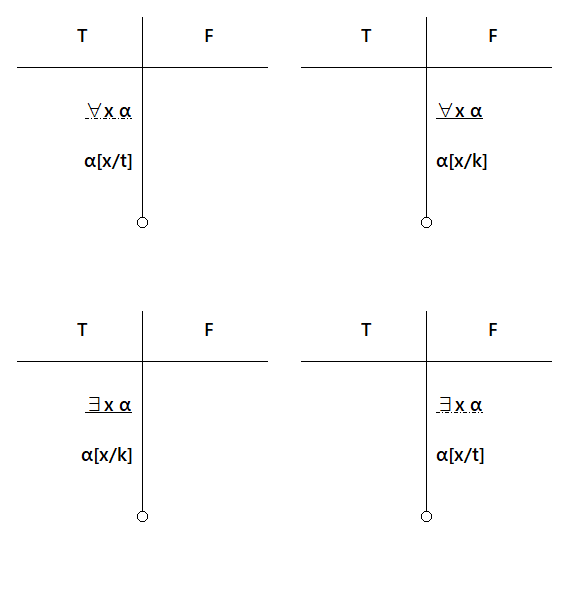
\includegraphics[scale=0.7]{images/Tableaux_Rules_Pred_Logic.png}
\caption{Tableaux Ableitungsregeln in klassischer Aussagenlogik}
\label{tableaux_class_pred_all_rules}
\end{center}
\end{figure}

\subsection{\label{tableaux_impl_descr}Nichtklassische Aussagenlogik}
Wie oben bereits erwähnt, bedarf es bei der Behandlung von Aussagen in nichtklassischer Logik einer anderen Abarbeitung der Junktoren.

In Abschnitt \ref{impl_in_intu} wurde bereits erwähnt, dass die nichtklassische Interpretation der Implikation die Herleitung eines Beweises aus einem bewiesenen Satz bedeutet. Das bedeutet, steht die Implikation $\alpha\rightarrow\beta$ auf der Folgerungsseite, wollen wir aus der Prämissenmenge $\delta$ auf einen Beweis von $\beta$ durch $\alpha$ schließen. Angenommen wir können dies beweisen, so ist es auch möglich von $\delta\cup\alpha$ auf $\beta$ zu schließen \cite{B62}.

Komplizierter und vor allem anders als in der klassischen Logik, ist die Ableitungsregel, wenn von der Prämissenmenge $\delta\cup\alpha\rightarrow\beta$ auf $\gamma$ geschlossen werden soll. Um $\alpha\rightarrow\beta$ in den Prämissen nutzen zu können, muss versucht werden $\beta$ aus $\alpha\rightarrow\beta$ und $\alpha$ zu schließen. Hierfür muss aber zuerst $\alpha$ aus $\delta\cup\alpha\rightarrow\beta$ geschlossen werden. Das anfängliche Problem wird also in zwei Subprobleme aufgeteilt \cite{B62}

\begin{itemize}
\item Beweise $\alpha$ (und dadurch $\beta$) aus $\delta\cup\alpha\rightarrow\beta$

\item Beweise $\gamma$ aus $\delta\cup\alpha\rightarrow\beta\cup\beta$
\end{itemize}

\textbf{Beachte:} Im ersten Subproblem ist $\gamma$ \textbf{nicht} in der Folgerungsmenge enthalten ist.

Es wird also erforderlich, die Aussagenmengen auf den beiden Seiten nach einer Ableitungsregel zu reduzieren. Semantisch wird dies im Tableau durch einen horizontalen Strich dargestellt unter dem beide Mengen neu definiert werden. Die Ableitung der Implikation wird in Abbildung \ref{tableaux_impl_ipc} dargestellt, P und C stehen hierbei für Premisses (dt.: Prämissen) und Conclusions (dt.: Folgerungen).

\begin{figure}
\begin{center}
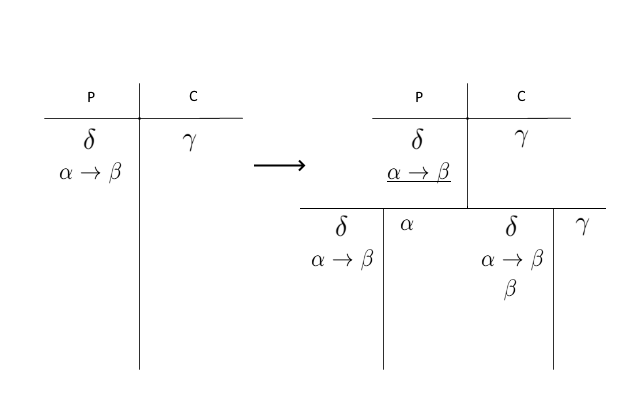
\includegraphics[scale=0.7]{images/Tableaux_Impl_IPC.png}
\caption{Tableau Ableitungsregel der Implikation in nichtklassischer Aussagenlogik}
\label{tableaux_impl_ipc}
\end{center}
\end{figure}

Bei Betrachtung der Negation, wird wie bereits in Abschnitt \ref{intu_non_proof_sentence} erwähnt wurde, die Negation $\neg\alpha$ durch $\alpha\rightarrow\perp$ substituiert. Bei einem automatischen Beweisverfahren, wird die Negation auf eine etwas andere Weise behandelt, wie in Abschnitt \textbf{EINFÜGEN!!!!} erarbeitet wird. Die sonstigen Ableitungsregeln sind allerdings Äquivalent zur klassischen Logik.

\subsection{Nichtklassische Prädikatenlogik}
Die nichtklassische Prädikatenlogik, welche Äquivalent zur klassischen Logik eine Erweiterung der nichtklassischen Aussagenlogik ist, bedarf einer Behandlung der Quantoren. Für den Allquantor in der Prämissenmenge bzw. den Existenzquantor in der Folgerungsmenge, gelten die Äquivalenten Regeln zur klassischen Prädikatenlogik. Aus $\forall$x $\alpha$ wird für jede Konstante t $\alpha$[x/t] zur Prämissenmenge hinzugefügt \cite{DGHP99}.

Steht jedoch $\forall$x $\alpha$ in der Folgerungsmenge, wird die Folgerungsmenge \{$\alpha$[x/a]\} abgeleitet, wobei a eine noch nicht existierende Konstante ist. Das heißt, ähnlich der Implikationsregel wird die Folgerungsmenge auf \{$\alpha$[x/a]\} reduziert \cite{DGHP99}.

Steht $\exists$x $\alpha$ in der Prämissenmenge $\delta$, wird die Prämissenmenge ($\delta$\textbackslash \{$\exists$x $\alpha$\})$\cup$\{$\alpha$[x/a]\} abgeleitet, wobei a eine noch nicht existierende Konstante ist. Die Folgerungsmenge wird für diese Regel also nicht berührt \cite{DGHP99}.

Die Ableitungsregeln sind in Abbildung \ref{tableaux_quantors_ifopl} dargestellt.

\begin{figure}
\begin{center}
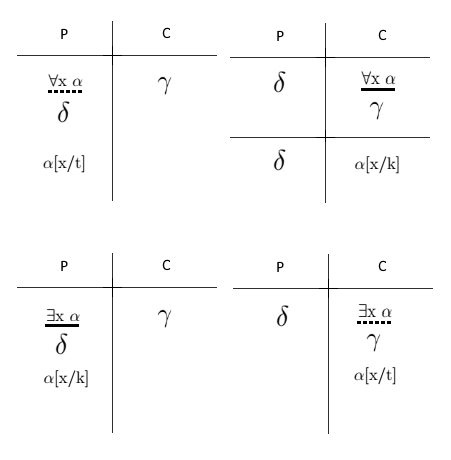
\includegraphics[scale=0.7]{images/Tableaux_Quantors_IFOPL.png}
\caption{Tableaux Ableitungsregeln der Quantoren in nichtklassischer Prädikatenlogik}
\label{tableaux_quantors_ifopl}
\end{center}
\end{figure}


